
\section{Einleitung zu den Klassendiagrammen}
In der Web-Application benutzen wir Typescript um in Javascript Typsicherheit zu gewähren. In den Diagrammen werden deshalb Typescript spezifische Typen und Utility Typen benutzt. Hierfür siehe Typescript Docs für Advanced Types und Utility Types: \\
\url{http://www.typescriptlang.org/docs/handbook/advanced-types.html} \\
\url{http://www.typescriptlang.org/docs/handbook/utility-types.html}

\begin{figure}[H]
	\hspace{-3cm}
	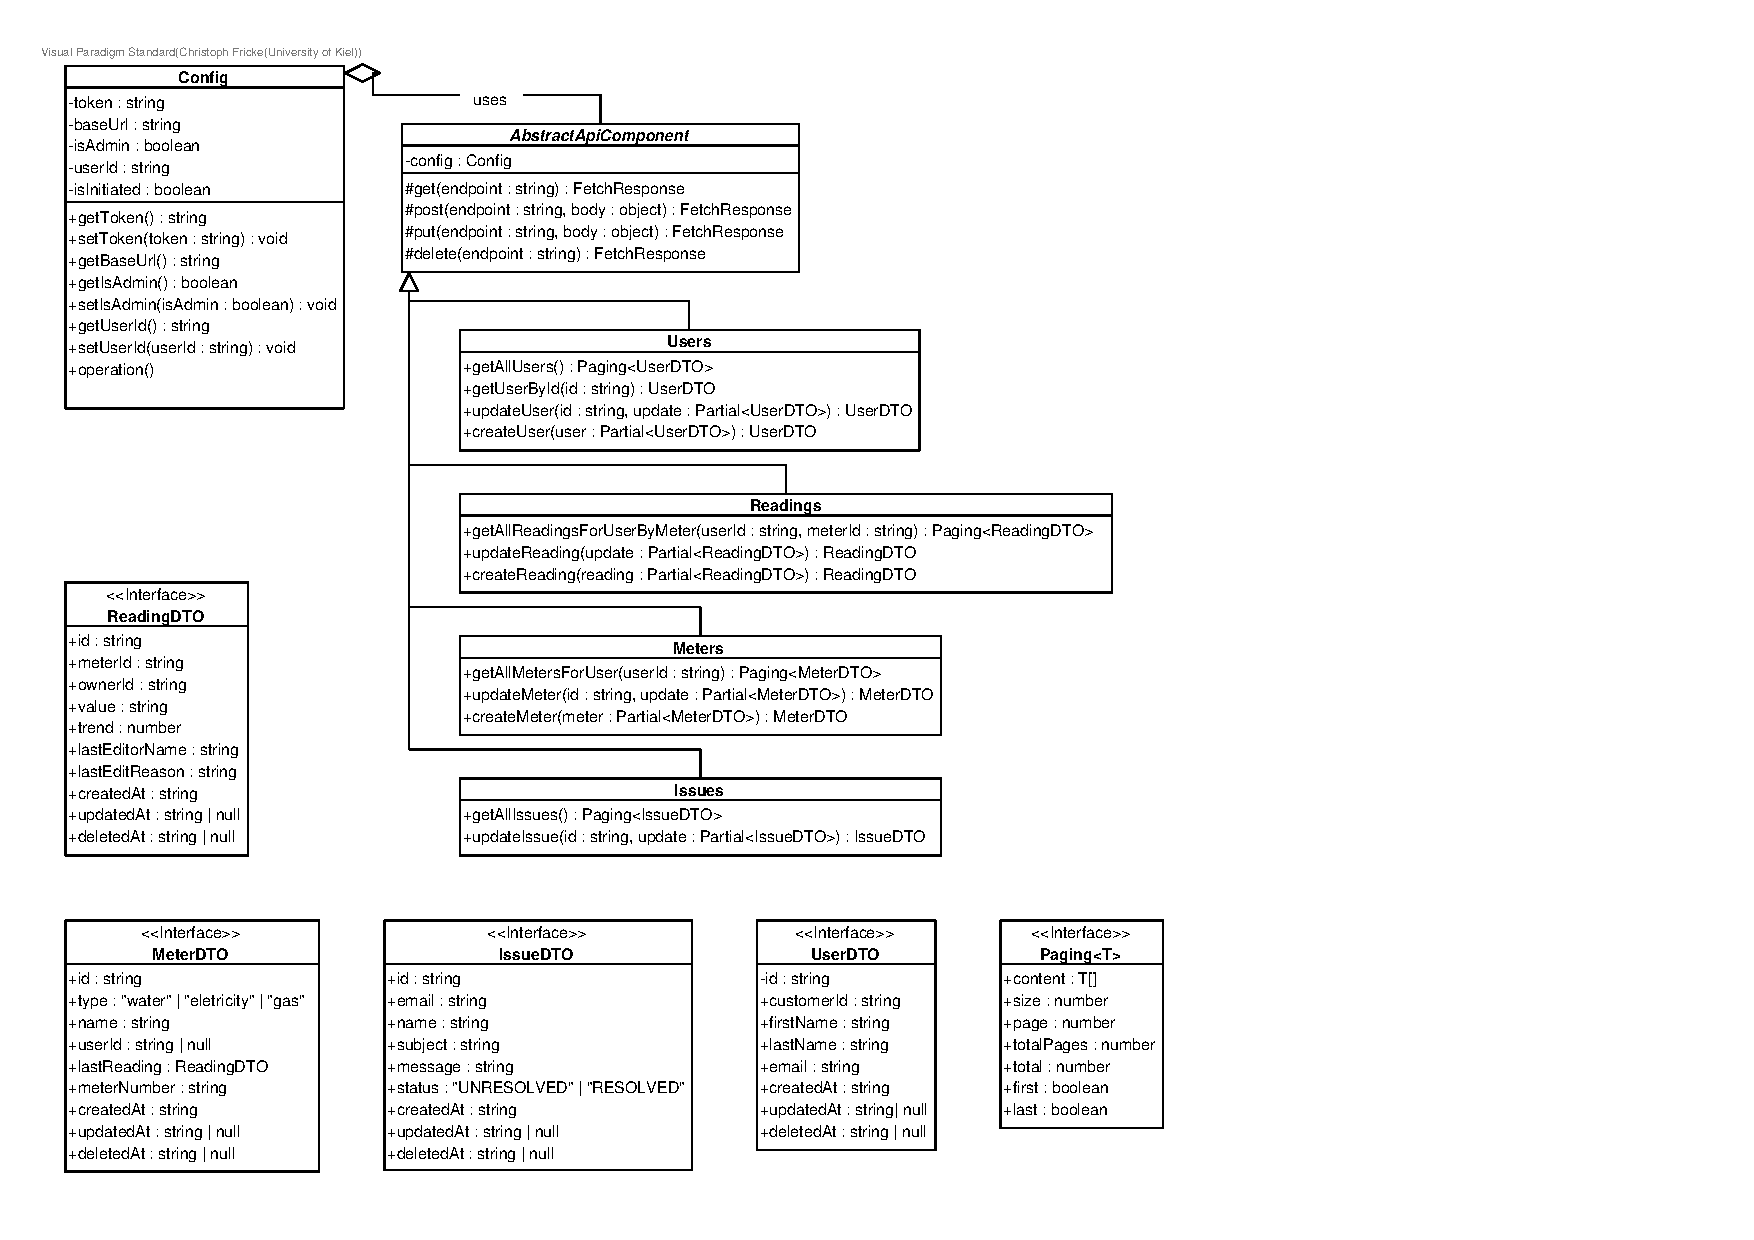
\includegraphics[scale = 0.9]{./img/diagrams/api-classDiagram}
	\caption{Klassendiagramm - API Abstraction}
\end{figure}
\newpage

\textbf{Beschreibung zum obrigen Klassendiagramm - API Abstraction.} \\ \\
Die verschiedenen DTO Interface sind Datentypen welche über die REST-Endpunkten verschickt werden. Sie dienen als Datentyp für Javascript Objekte in Typescript. In der API-Abstraction halten wir eine eigene Config-Klasse, damit Komponenten welche die Abstraction benutzen, nicht bei jedem Aufruf den Token und die Base-URL mitgeben müssen. Dadurch muss die Config nur einmal initialisiert werden, sobald der Benutzer die Website lädt. \\ \\
Eine Abstrakte Klasse stellt konfigurierte Netzwerkfunktionen für die spezialisierten Klassen zur Verfügung, sodass die Methode zum erstellen von Netzwerk Anfragen (fetch oder axios) leichter ausgetauscht werden kann. \\
Die spezialisierten API Componenten + Config sind Singletons. Eine index Datei in den API Package exportiert für
jede Klasse ein Object wodurch auf einfache Art und Weise ein Singleton Pattern in JS realisiert werden kann.
Zum Testen kann weiterhin die Klasse importiert werden, sodass z.b. von der Config in jeden Test ein neues
Objekt verfügbar ist. Dieses Verhalten wäre auch durch Mocking erreichbar, ist jedoch aufwendiger umzusetzen und erzeugt mehr Overhead. \\

\begin{table}[H]
	\centering
	\begin{tabularx}{\textwidth}{X X}
		\rowcolor[HTML]{C0C0C0} 
		\textbf{Klassenname} & \textbf{Aufgabe} \\
		Config& Speichert API Access Informationen wie Token und Base-URL. Auf diese kann nicht zugegriffen werden, bevor die Config initialisiert wurde.  \\
		\rowcolor[HTML]{E7E7E7} 
		AbstractApiComponent & Stellt konfigurierte Netzwerkfunktionen für die spezialisierten Klassen zur Verfügung. \\
		Users & Beinhaltet Funktionen um auf die Rest-Endpunkte zuzugreifen, welche inhaltlich zu den Benutzern gehören. \\
		\rowcolor[HTML]{E7E7E7} 
		Readings & Beinhaltet Funktionen um auf die Rest-Endpunkte zuzugreifen, welche inhaltlich zu den Zählerstände gehören. \\
		Meters & Beinhaltet Funktionen um auf die Rest-Endpunkte zuzugreifen, welche inhaltlich zu den Zählern gehören. \\
		\rowcolor[HTML]{E7E7E7} 
		Issues & Beinhaltet Funktionen um auf die Rest-Endpunkte zuzugreifen, welche inhaltlich zu den Tickets gehören. \\
	\end{tabularx}
	\caption{Klassenbeschreibung - API Abstraction}
	\label{table:klassenbeschreibung-api Abstraction}
\end{table}


\begin{figure}[H]
	\hspace{-3cm}
	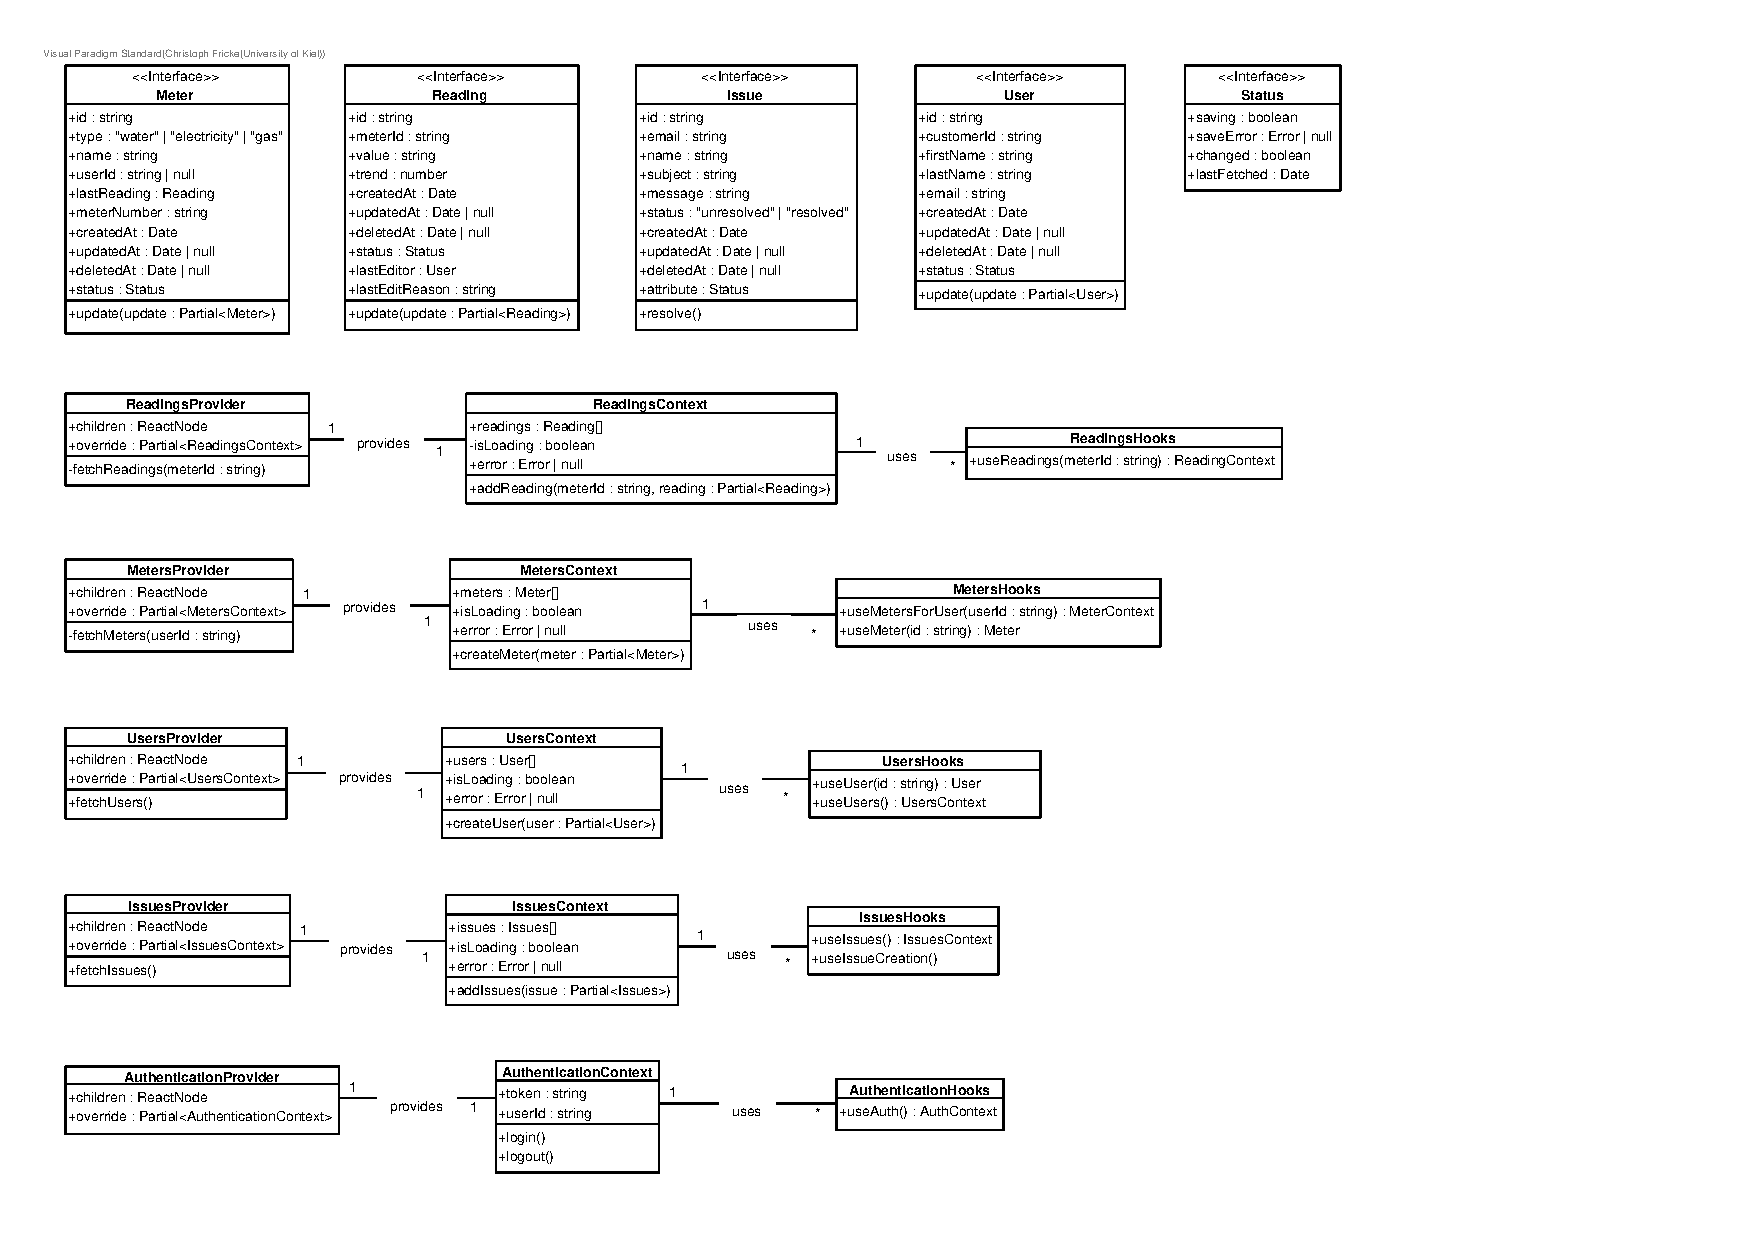
\includegraphics[scale = 0.9]{./img/diagrams/providers-classDiagram}
	\caption{Klassendiagramm - Provider}
\end{figure}
\newpage

\textbf{Beschreibung zum obrigen Klassendiagramm - Provider.} \\ \\
Für das Klassendiagramm für die Provider ist es wichtig \href{https://reactjs.org/docs/context.html}{React Context} zu verstehen.  Der Override in den Providern erlaubt es uns den Context in Tests auszutauschen. Dadurch können Components, deren Kinder oder diese selber einen Access Hook  benutzen, 
getestet werden, ohne das der Hook gemockt werden muss. \href{https://reactjs.org/docs/hooks-intro.html}{Hooks} sind eine React-Funktionalität um Logik innerhalb von Componenten zu abstrahieren und wiederzuverwenden. Ein Context wird hier als Klasse dargestellt. In Wahrheit ist es aber ein Objekt, 
welches von React verwaltet wird. Dadurch werden konsumierende Components bei Updates automatisch neu gerendert. Das Ganze ist vergleichbar mit einem Observer Pattern. \\
Die Hook Klassen existieren nur im Diagramm. Im Quellcode sind es nur die aufgelisteten Hooks, welche von den UI Components benutzt werden können um Zugriff auf die Contexte zu bekommen. Die Hooks dienen damit als Fassade, sodass die React Contexte auch durch Redux für das globale State Management ersetzt werden könnten.
Provider Components bringen die verschiedene Contexte in den React-Tree, damit diese für die Hooks in den UI Components zur Verfügung stehen.\\
Die Interface welche im Context gehalten werden, sind erweiterte DTO interface welche zusätzliche interne Informationen speichern.

\begin{table}[H]
	\centering
	\begin{tabularx}{\textwidth}{X X}
		\rowcolor[HTML]{C0C0C0} 
		\textbf{Klassenname} & \textbf{Aufgabe} \\
		*Context & Conxtexte stellen ihren zugehörige Informationen global zur Verfügung.  \\
		\rowcolor[HTML]{E7E7E7} 
		*Provider & Die Provider rendern ihren zugehörigen Context in den React-Tree. \\
		*Hooks & Hooks sind Zugriffsfunktionen als Fassade für die zugehörigen Contexte, damit die Componenten nicht direkt auf den Context zugreifen. \\
	\end{tabularx}
	\caption{Klassenbeschreibung - Provider}
	\label{table:klassenbeschreibung-provider}
\end{table}
\newpage

\begin{figure}[H]
	\hspace{-3cm}
	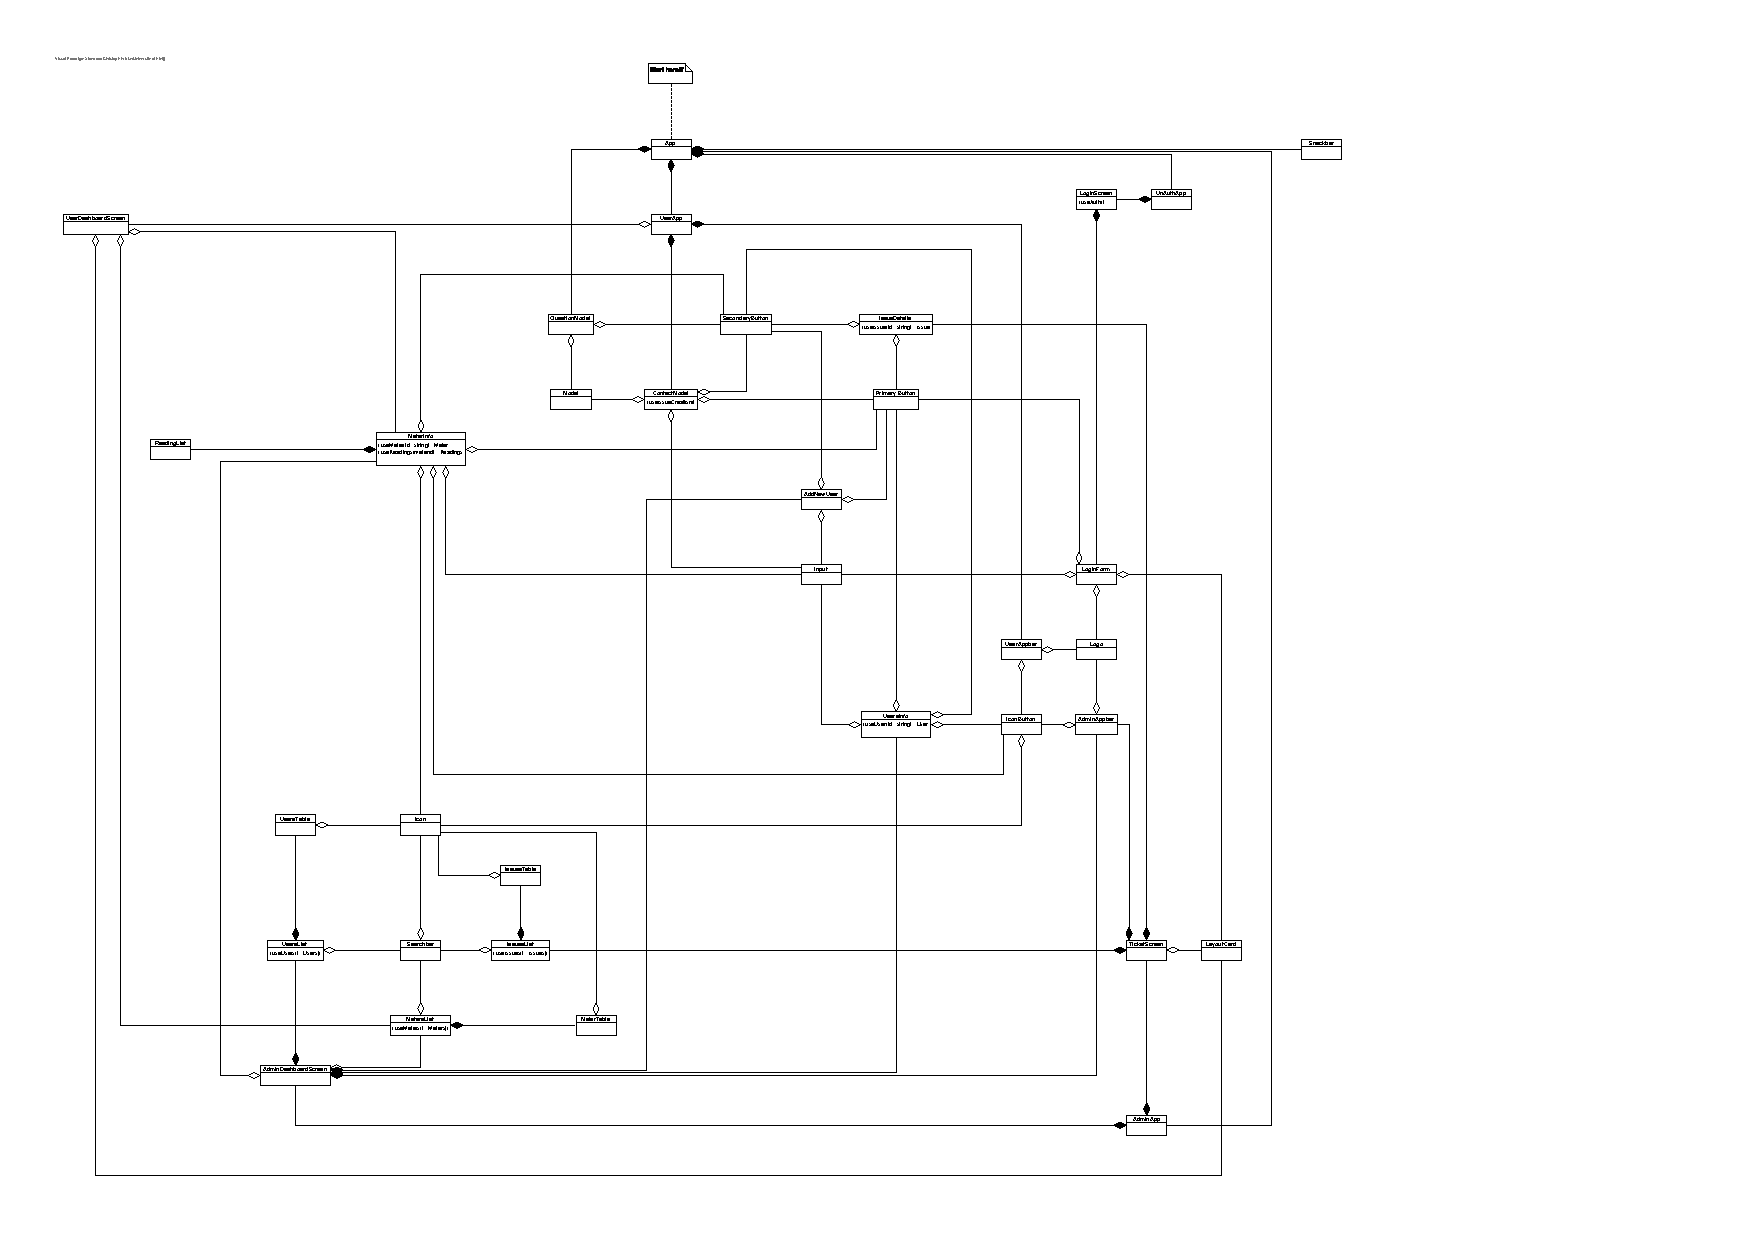
\includegraphics[scale = 0.9]{./img/diagrams/web-class}
	\caption{Klassendiagramm - Benutzeroberfläche Componenten}
\end{figure}
\newpage

\textbf{Beschreibung zum obrigen Klassendiagramm - Benutzeroberfläche Componenten} \\ \\
Alle Klassen aus dem Diagramm sind \href{https://reactjs.org/docs/components-and-props.html}{React-Componenten}. Damit es übersichtlicher ist, haben wir die Properties und internen State sowie die Kardinalitäten der Associationen rausgelassen und nur Hooks aus der Provider-Schicht hinzugefügt wo wir vermuten auf den globalen State zuzugreifen. \\ \\
Allgemein bestehen die Benutzeroberflächen aus Kompositionen von UI Componenten welche von React in den HTML-DOM gerendert werden. 
 
\begin{table}[H]
	\centering
	\begin{tabularx}{\textwidth}{X X}
		\rowcolor[HTML]{C0C0C0} 
		\textbf{Klassenname} & \textbf{Aufgabe} \\
		App & App ist die Hauptkomponente welche in den HTML-DOM gerendert wird. Basierend auf den Status des Benutzers, rendert diese entweder die 	User-App, die Admin-App oder die Unauth-App. \\
		\rowcolor[HTML]{E7E7E7} 
		Layout Card & Die Layout Card rendert eine weiße Box welche als Container für ihre inneren Componenten dient.  \\
		Snackbar & Die Snackbar sind kleine Pop-up Benachrichtigungen welche dem Benutzer Statusmeldungen mitteilen.  \\
		\rowcolor[HTML]{E7E7E7} 
		UsersList & Die UsersList rendert eine Liste mit Suchbar von allen Benutzern. \\
		MetersList & Die MetersList rendert eine Liste mit Suchbar von allen Zählern eines Benutzers. \\
		\rowcolor[HTML]{E7E7E7} 
		IssuesList & Die IssuesList rendert eine Liste mit Suchbar von allen Tickets.\\
		UsersInfo & Enthält Informationen über die Benutzer und die Möglichkeit diese zu editieren. \\
		\rowcolor[HTML]{E7E7E7} 
		IssueDetails & Enthält eine Detaillierte Ansicht über ein Ticket und Interaktions möglichkeiten.\\
		MeterInfo & Enthält Informationen über einen Zähler und seine Zählerstände.
	\end{tabularx}
	\caption{Klassenbeschreibung - Benutzeroberfläche Componenten}
	\label{table:klassenbeschreibung-ui}
\end{table}

\section{Klassendiagramme - Back-End}
\begin{figure}[H]
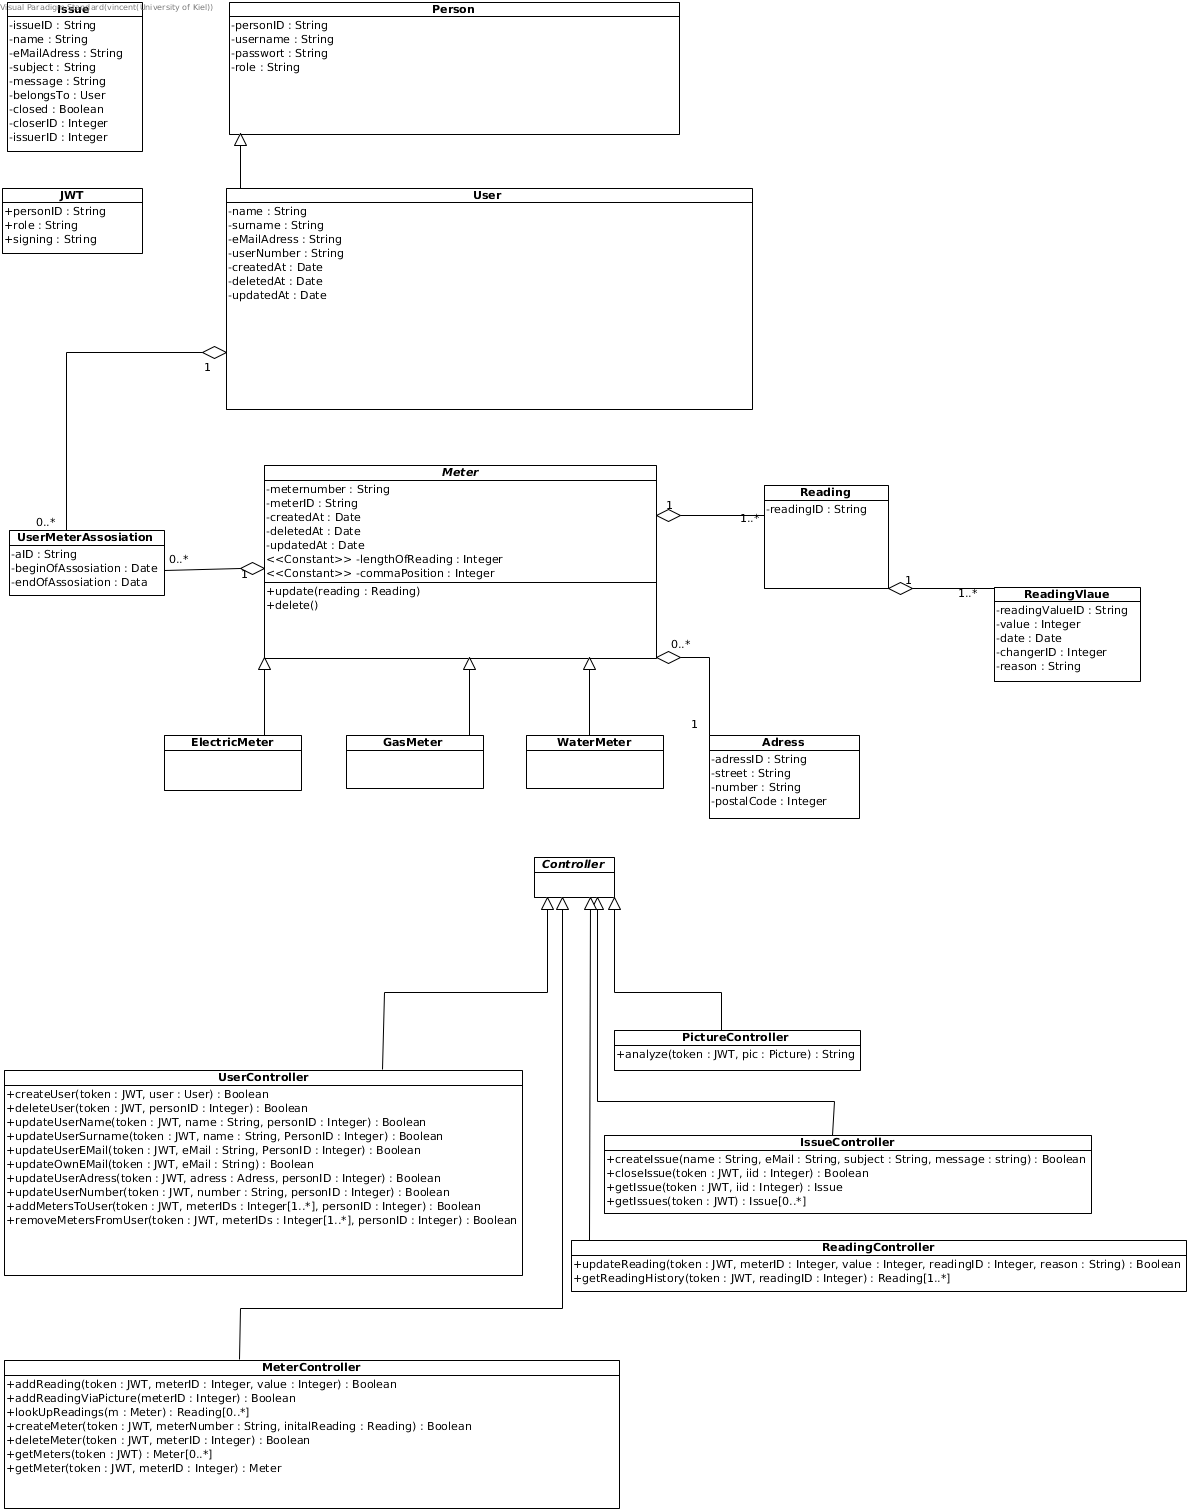
\includegraphics[width=15cm]{img/diagrams/backend-class-diagram}\\
\caption{Klassendiagramm - Back-End}
\end{figure}
Bei allen Objekten, die Entities des Models darstellen (Person, User, UserMeterAssociation, Meter, Reading, ReadingValue, Adress, Issue), handelt es sich um Spring Entity-Objekte.
Die normalerweise anfallenden Klassen (z.B. Repository-Klassen) werden zwar generiert, aber zu Übersichtszwecken nicht im Diagramm aufgeführt.\\
JWT steht für JSON Web Token. 
JWTs werden genutzt, um bei Anfragen an die REST-API User und Administratoren zu authentifizieren. Die REST-API wird durch den Controller bereitgestellt.
Man kann daher auch aus jeder Anfrage, die einen JWT enthält, einen konkreten User herauslesen. 
Da es sich um ein JSON-Objekt handelt, wird es intern nur als String wahrgenommen, aber zur Übersicht im Diagramm wurde es mit dem geplantem Inhalt als Java-Klasse aufgeführt.\\
Da Kunden aus einer Wohnung ausziehen können und neue Kunden dort einziehen können, benötigen Kunden und Zähler eine Komponente oder Funktion, welche einen Zähler zu einem Gewissen Zeitpunkt einem Kunden zuordnet. 
Zu diesem Zweck existiert die UserMeterAssosiation.\\
Ein Zähler besitzt mindestens einen aktuellen Zählerstand und gegebenenfalls mehrere alte Zählerstände, sowie eine Adresse, an der er montiert ist.\\
Das Attribut lengthOfReading wird von den konkreten Zählern geerbt und beschreibt, welche Länge eine Eingabe dieser Zählerart besitzt. Das Attribut commePosition besagt dabei, wie viele Nachkommastellen es gibt.\\
Ein Zählerstand hat mindestens einen Wert der beim Ablesen angegeben wird. 
Da er aber unter Umständen von Administratoren geändert werden kann, werden zusätzlich alle Versionen des Zählerstandes inklusive der Person die ihn verändert hat, ebenfalls wird der Grund für die Änderung gespeichert.
Beim Erstellen eines Zählerstandes wird ein ReadingValue aus dem tatsächlichen Stand des Zählers und Default-Werten für Grund und Ersteller generiert.\\
Die Controller dienen zum Auslesen und Manipulieren der Daten des Models. 
Die Controller sind jeweils darauf spezialisiert die Anfragen von Nutzern, Zählern oder Einträgen zu händeln.

\section{Klassendiagramme - App}
Die App ist intern in eine View- und eine Model/Controller-Komponente aufgeteilt. Es folgen Klassendiagramme für die 2 Komponenten.
\begin{figure}[H]
\centering
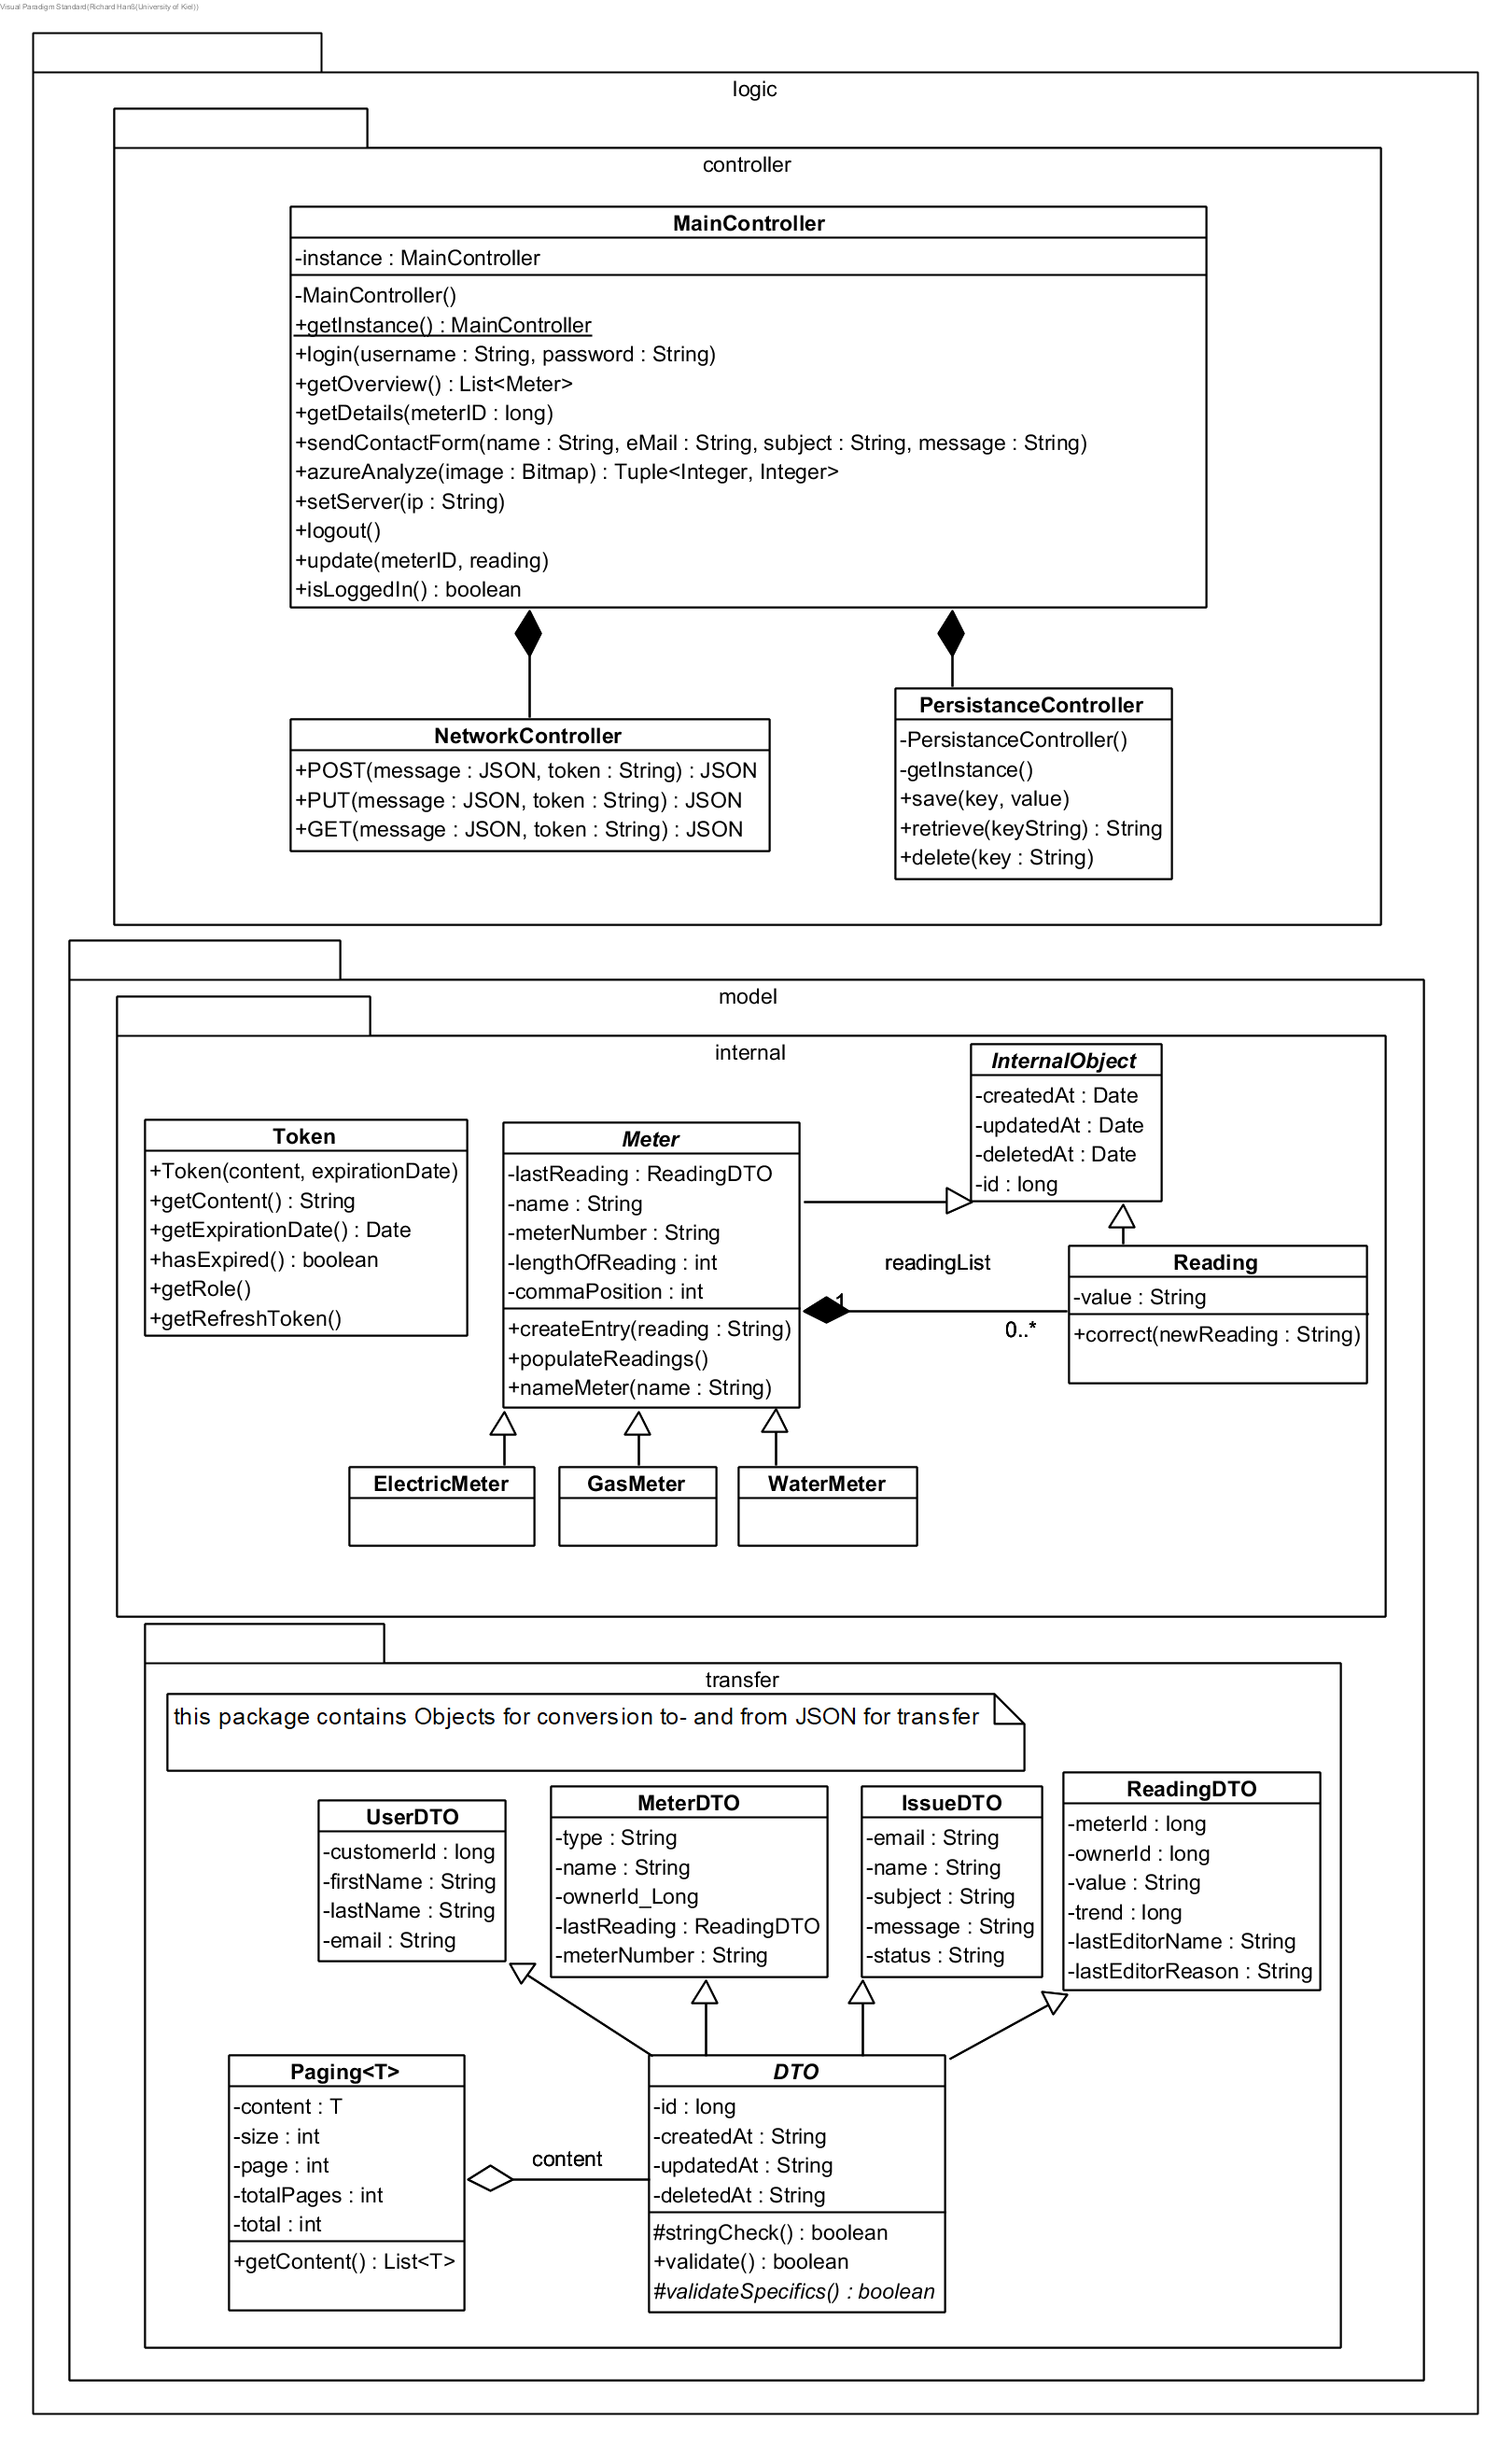
\includegraphics[height=20cm,width=15cm]{img/diagrams/Android-Class-Diagram-Logic}\\
\caption{Logik der App}
\end{figure}


\subsection*{Erklärung - Model \& Controller der App}
Im Package 'logic' befinden sich die Packages 'model' und 'controller'.
Klassen im Controller-Package sind verantwortlich fürs tatsächliche Ausführen der Operationen, die vom User über Interaktion mit den Views gestartet werden. \\ Die Singleton-Klasse MainController ist hier erster Ansprechpunkt für die Views und stellt Methoden zum Ein- und Ausloggen, Analysieren von Bildern, Fetchen von Zählern, Senden von Kontaktanfragen und ändern vom zu benutzendem Server. \\ Der MainController benutzt zum senden von HTTP-Requests den NetworkController und zum Speichern von persistenten Daten (wie z.b. OAuth Token) den PersistanceController.
Das Model ist in 2 Packages unterteilt. 'internal' enthält Objekte, die den Views zur Anzeige übergeben werden, sowie eine Repräsentation des OAuth-Tokens. \\ Im 'transfer' package befinden sich Klassen, die identisch zu den über REST zu übertragenden JSON Objekten aufgebaut sind. Sie werden über eine Library von- und zu JSON konvertiert werden.

\begin{figure}[H]
\hspace{-1cm}
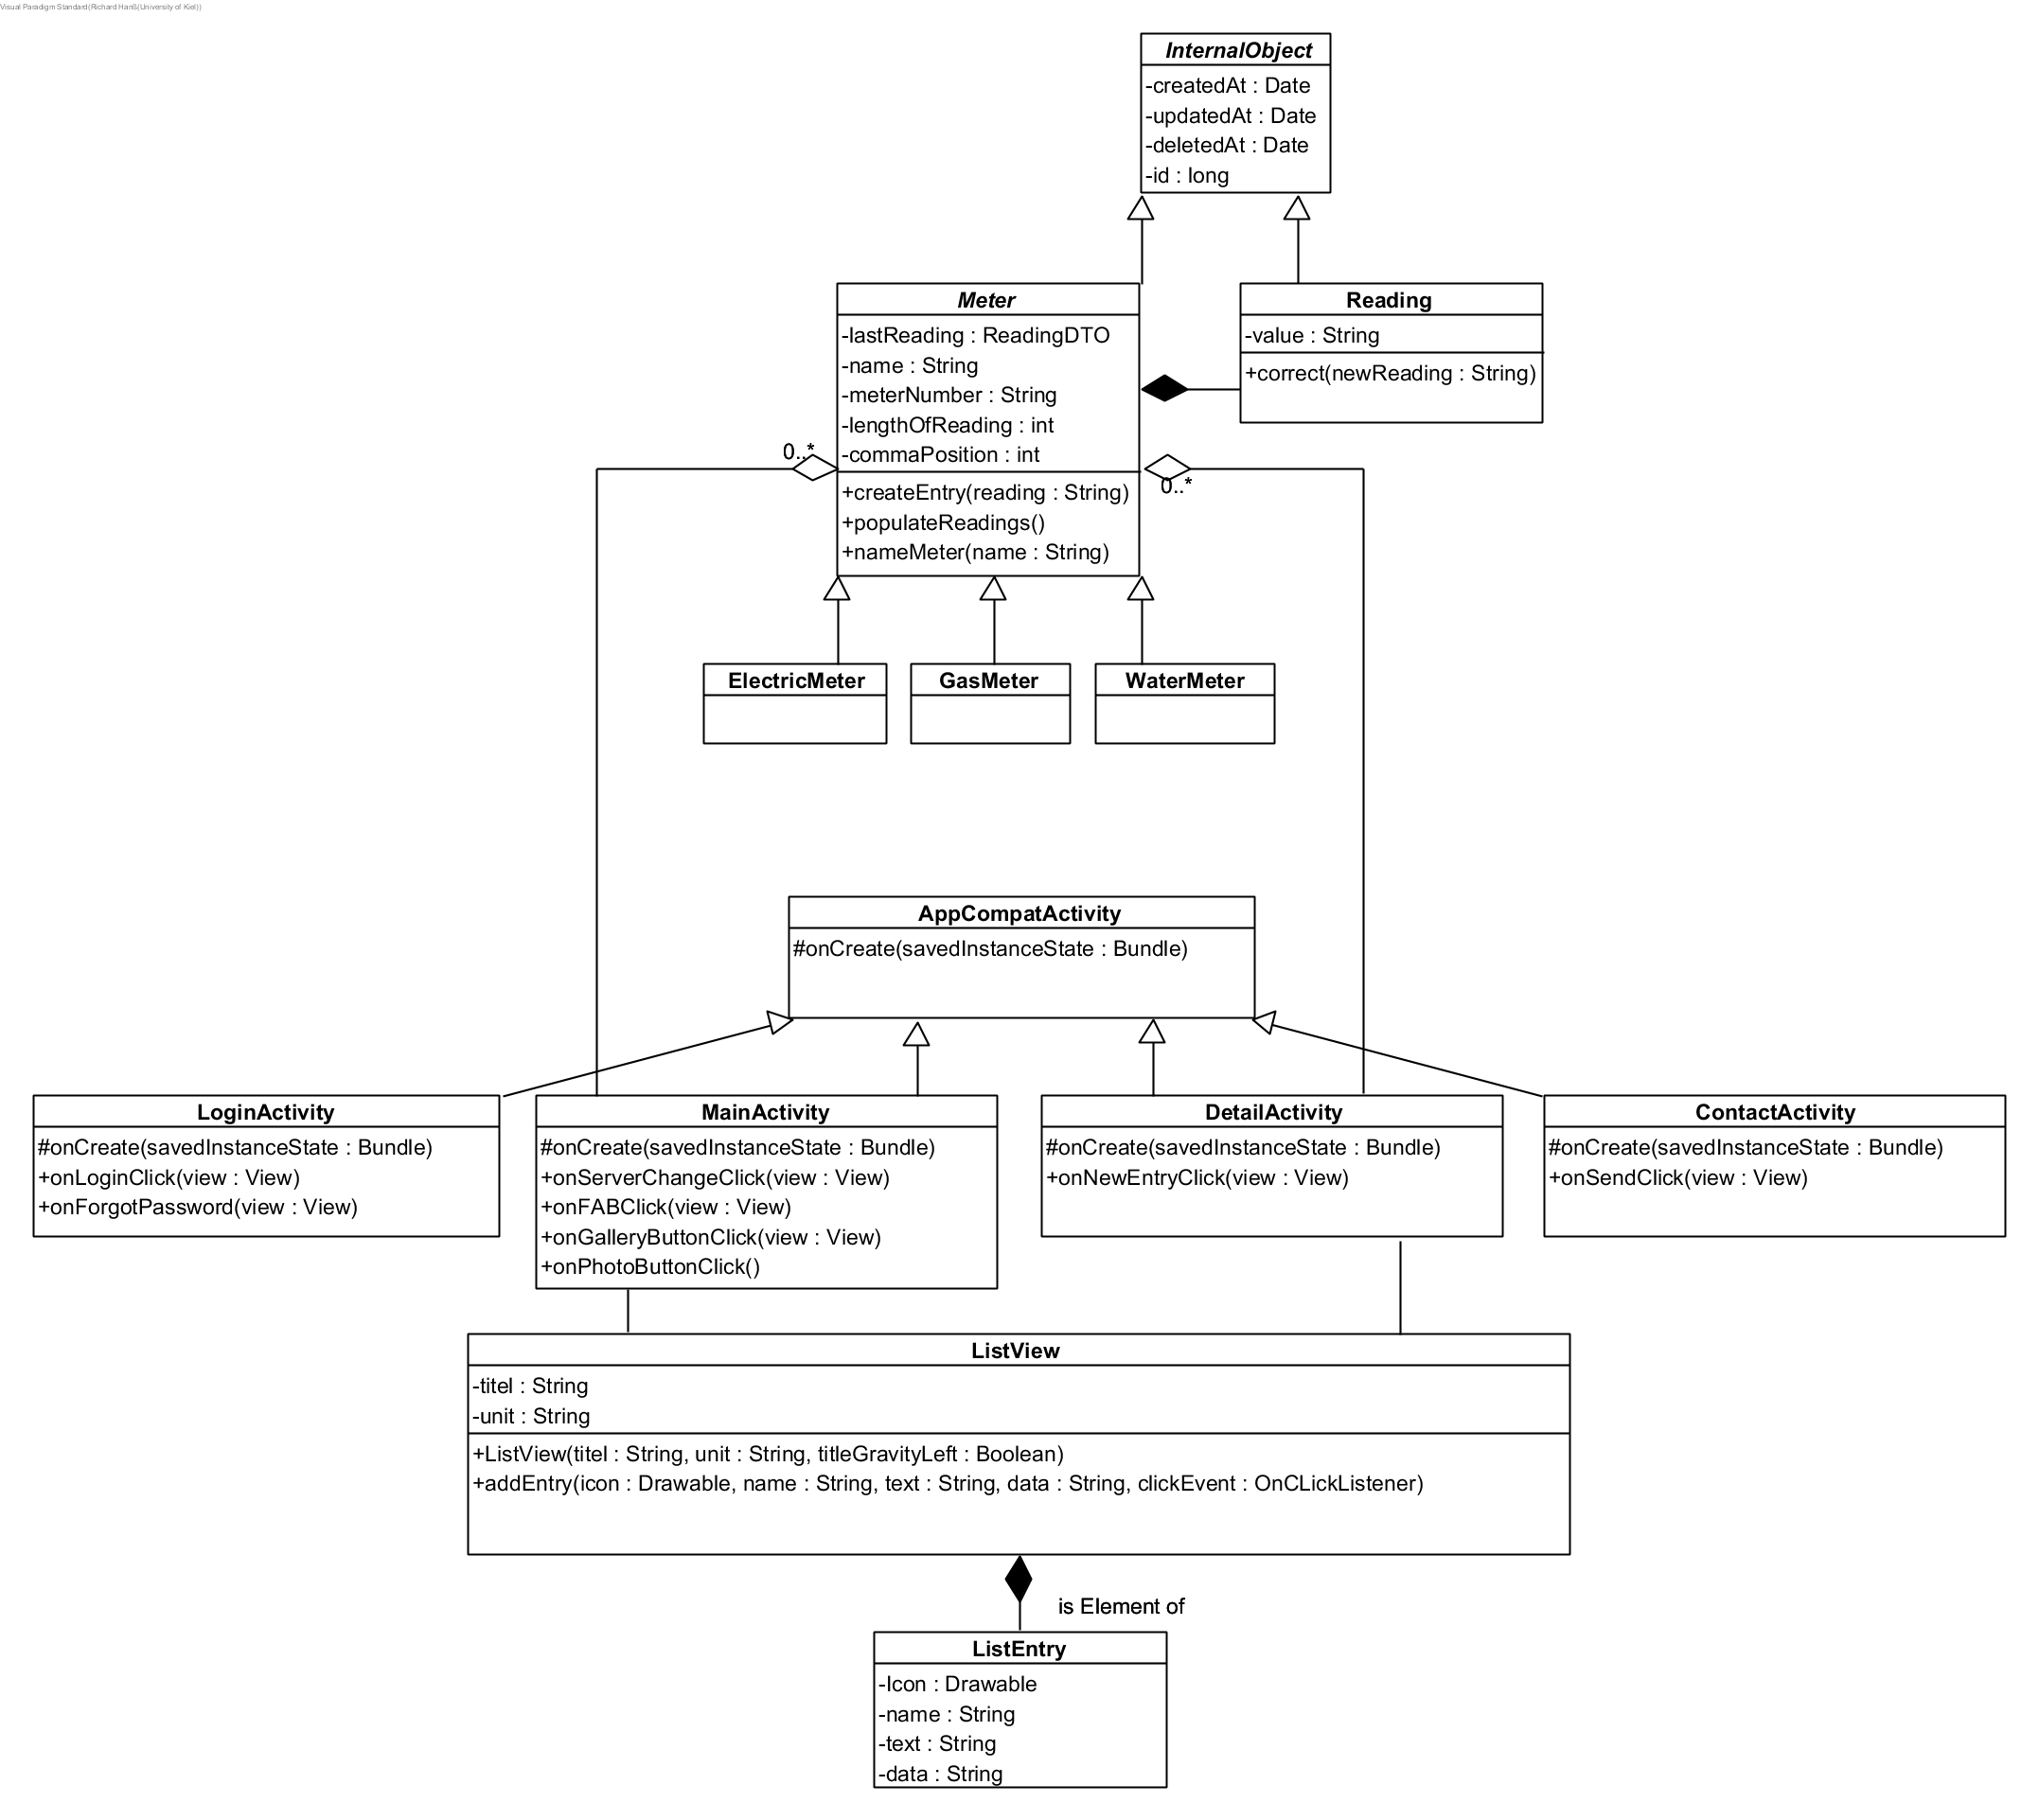
\includegraphics[height=14cm]{img/diagrams/Android-Class-Diagram-View}\\
\caption{Android View}
\end{figure}

\subsection*{Erklärung - View der App}
\begin{tabularx}{15cm}{XX}
	\hline
	Meter/InternalObject/Reading & Die hier aufgeführte Meter Klasse ist dieselbe, die auch in dem Logikdiagram dargestellt ist. \\ \hline
	ElectricMeter/GasMeter/WaterMeter & Die hier aufgeführte Meter Klasse ist dieselbe, die auch in dem Logikdiagram dargestellt ist. \\ \hline
	AppCompatActivity & Diese Klasse ist standartmäßig die Superklasse von allen Activities in Android Studio \\ \hline
	LoginActivity & Diese Activity stellt UI Elemente bereit, die es dem Nutzer erlauben sich anzumelden. \\ \hline
	MainActivity & Auf dieser Activity kann der Nutzer seine Zähler und einige Zählerstände einsehen, sowie auf sie zugreifen. \\ \hline
	DetailActivity & Auf dieser Activity kann der Nutzer Zählerstände hinzufügen und einsehen. \\ \hline
	IssueActivity & Auf dieser Activity kann der Nutzer einen Admin kontaktieren, falls er ein Problem hat. \\ \hline
	ListView & Diese Klasse erleichtert das hinzufügen und maintainen von Listen in der ManActivity und DetailActivity. \\ \hline
	ListEntry & Diese Klasse stellt einen Listeneintrag dar. 
\end{tabularx}

